\documentclass[]{book}
\usepackage{lmodern}
\usepackage{amssymb,amsmath}
\usepackage{ifxetex,ifluatex}
\usepackage{fixltx2e} % provides \textsubscript
\ifnum 0\ifxetex 1\fi\ifluatex 1\fi=0 % if pdftex
  \usepackage[T1]{fontenc}
  \usepackage[utf8]{inputenc}
\else % if luatex or xelatex
  \ifxetex
    \usepackage{mathspec}
  \else
    \usepackage{fontspec}
  \fi
  \defaultfontfeatures{Ligatures=TeX,Scale=MatchLowercase}
\fi
% use upquote if available, for straight quotes in verbatim environments
\IfFileExists{upquote.sty}{\usepackage{upquote}}{}
% use microtype if available
\IfFileExists{microtype.sty}{%
\usepackage{microtype}
\UseMicrotypeSet[protrusion]{basicmath} % disable protrusion for tt fonts
}{}
\usepackage[margin=1in]{geometry}
\usepackage{hyperref}
\hypersetup{unicode=true,
            pdftitle={life's work},
            pdfauthor={Charles T. Gray},
            pdfborder={0 0 0},
            breaklinks=true}
\urlstyle{same}  % don't use monospace font for urls
\usepackage{natbib}
\bibliographystyle{apalike}
\usepackage{color}
\usepackage{fancyvrb}
\newcommand{\VerbBar}{|}
\newcommand{\VERB}{\Verb[commandchars=\\\{\}]}
\DefineVerbatimEnvironment{Highlighting}{Verbatim}{commandchars=\\\{\}}
% Add ',fontsize=\small' for more characters per line
\usepackage{framed}
\definecolor{shadecolor}{RGB}{248,248,248}
\newenvironment{Shaded}{\begin{snugshade}}{\end{snugshade}}
\newcommand{\AlertTok}[1]{\textcolor[rgb]{0.94,0.16,0.16}{#1}}
\newcommand{\AnnotationTok}[1]{\textcolor[rgb]{0.56,0.35,0.01}{\textbf{\textit{#1}}}}
\newcommand{\AttributeTok}[1]{\textcolor[rgb]{0.77,0.63,0.00}{#1}}
\newcommand{\BaseNTok}[1]{\textcolor[rgb]{0.00,0.00,0.81}{#1}}
\newcommand{\BuiltInTok}[1]{#1}
\newcommand{\CharTok}[1]{\textcolor[rgb]{0.31,0.60,0.02}{#1}}
\newcommand{\CommentTok}[1]{\textcolor[rgb]{0.56,0.35,0.01}{\textit{#1}}}
\newcommand{\CommentVarTok}[1]{\textcolor[rgb]{0.56,0.35,0.01}{\textbf{\textit{#1}}}}
\newcommand{\ConstantTok}[1]{\textcolor[rgb]{0.00,0.00,0.00}{#1}}
\newcommand{\ControlFlowTok}[1]{\textcolor[rgb]{0.13,0.29,0.53}{\textbf{#1}}}
\newcommand{\DataTypeTok}[1]{\textcolor[rgb]{0.13,0.29,0.53}{#1}}
\newcommand{\DecValTok}[1]{\textcolor[rgb]{0.00,0.00,0.81}{#1}}
\newcommand{\DocumentationTok}[1]{\textcolor[rgb]{0.56,0.35,0.01}{\textbf{\textit{#1}}}}
\newcommand{\ErrorTok}[1]{\textcolor[rgb]{0.64,0.00,0.00}{\textbf{#1}}}
\newcommand{\ExtensionTok}[1]{#1}
\newcommand{\FloatTok}[1]{\textcolor[rgb]{0.00,0.00,0.81}{#1}}
\newcommand{\FunctionTok}[1]{\textcolor[rgb]{0.00,0.00,0.00}{#1}}
\newcommand{\ImportTok}[1]{#1}
\newcommand{\InformationTok}[1]{\textcolor[rgb]{0.56,0.35,0.01}{\textbf{\textit{#1}}}}
\newcommand{\KeywordTok}[1]{\textcolor[rgb]{0.13,0.29,0.53}{\textbf{#1}}}
\newcommand{\NormalTok}[1]{#1}
\newcommand{\OperatorTok}[1]{\textcolor[rgb]{0.81,0.36,0.00}{\textbf{#1}}}
\newcommand{\OtherTok}[1]{\textcolor[rgb]{0.56,0.35,0.01}{#1}}
\newcommand{\PreprocessorTok}[1]{\textcolor[rgb]{0.56,0.35,0.01}{\textit{#1}}}
\newcommand{\RegionMarkerTok}[1]{#1}
\newcommand{\SpecialCharTok}[1]{\textcolor[rgb]{0.00,0.00,0.00}{#1}}
\newcommand{\SpecialStringTok}[1]{\textcolor[rgb]{0.31,0.60,0.02}{#1}}
\newcommand{\StringTok}[1]{\textcolor[rgb]{0.31,0.60,0.02}{#1}}
\newcommand{\VariableTok}[1]{\textcolor[rgb]{0.00,0.00,0.00}{#1}}
\newcommand{\VerbatimStringTok}[1]{\textcolor[rgb]{0.31,0.60,0.02}{#1}}
\newcommand{\WarningTok}[1]{\textcolor[rgb]{0.56,0.35,0.01}{\textbf{\textit{#1}}}}
\usepackage{longtable,booktabs}
\usepackage{graphicx,grffile}
\makeatletter
\def\maxwidth{\ifdim\Gin@nat@width>\linewidth\linewidth\else\Gin@nat@width\fi}
\def\maxheight{\ifdim\Gin@nat@height>\textheight\textheight\else\Gin@nat@height\fi}
\makeatother
% Scale images if necessary, so that they will not overflow the page
% margins by default, and it is still possible to overwrite the defaults
% using explicit options in \includegraphics[width, height, ...]{}
\setkeys{Gin}{width=\maxwidth,height=\maxheight,keepaspectratio}
\IfFileExists{parskip.sty}{%
\usepackage{parskip}
}{% else
\setlength{\parindent}{0pt}
\setlength{\parskip}{6pt plus 2pt minus 1pt}
}
\setlength{\emergencystretch}{3em}  % prevent overfull lines
\providecommand{\tightlist}{%
  \setlength{\itemsep}{0pt}\setlength{\parskip}{0pt}}
\setcounter{secnumdepth}{5}
% Redefines (sub)paragraphs to behave more like sections
\ifx\paragraph\undefined\else
\let\oldparagraph\paragraph
\renewcommand{\paragraph}[1]{\oldparagraph{#1}\mbox{}}
\fi
\ifx\subparagraph\undefined\else
\let\oldsubparagraph\subparagraph
\renewcommand{\subparagraph}[1]{\oldsubparagraph{#1}\mbox{}}
\fi

%%% Use protect on footnotes to avoid problems with footnotes in titles
\let\rmarkdownfootnote\footnote%
\def\footnote{\protect\rmarkdownfootnote}

%%% Change title format to be more compact
\usepackage{titling}

% Create subtitle command for use in maketitle
\newcommand{\subtitle}[1]{
  \posttitle{
    \begin{center}\large#1\end{center}
    }
}

\setlength{\droptitle}{-2em}

  \title{life's work}
    \pretitle{\vspace{\droptitle}\centering\huge}
  \posttitle{\par}
  \subtitle{ruminations on the inelegant art of failing forwards}
  \author{\href{http://cantabile.rbind.io/about.html}{Charles T. Gray}}
    \preauthor{\centering\large\emph}
  \postauthor{\par}
      \predate{\centering\large\emph}
  \postdate{\par}
    \date{\emph{perennial work in progress} Tuesday 2 April 2019}

\usepackage{booktabs}

\begin{document}
\maketitle

{
\setcounter{tocdepth}{1}
\tableofcontents
}
\hypertarget{preamble}{%
\chapter{preamble}\label{preamble}}

What if one practices mathematical science like music?

My goal is to spend four hours a day on \protect\hyperlink{work-with-intent}{work with intent}.

For a sanity, efficiency, and inspiration, I intend to balance my time between categories:

\begin{itemize}
\tightlist
\item
  research, \(\varphi\);
\item
  skills, \(\theta\);\\
\item
  busywork, \(\psi\); and
\item
  wellness, \(\pi\)
\end{itemize}

\hypertarget{what-is-this}{%
\chapter{what is this?}\label{what-is-this}}

This manuscript is a triptych of

\begin{itemize}
\tightlist
\item
  \protect\hyperlink{analysis}{analysis} of my productivity data
\item
  \protect\hyperlink{rituals}{rituals} rituals to facillitate flow in practicing mathematical science
\item
  \protect\hyperlink{ruminations}{ruminations} a reminder to self about why I chose what I did
\end{itemize}

\hypertarget{version}{%
\section{\texorpdfstring{\protect\hyperlink{mindfulness}{version}}{version}}\label{version}}

Captain Marvel GIF from Captainmarvel GIFs

\begin{longtable}[]{@{}lll@{}}
\toprule
operation & instantiated & last updated\tabularnewline
\midrule
\endhead
phoenix & Tuesday 2 April 2019 & Tuesday 2 April 2019\tabularnewline
\bottomrule
\end{longtable}

\hypertarget{analysis}{%
\chapter{analysis}\label{analysis}}

\hypertarget{workload-intensity-goals-achieved}{%
\section{workload intensity goals achieved}\label{workload-intensity-goals-achieved}}

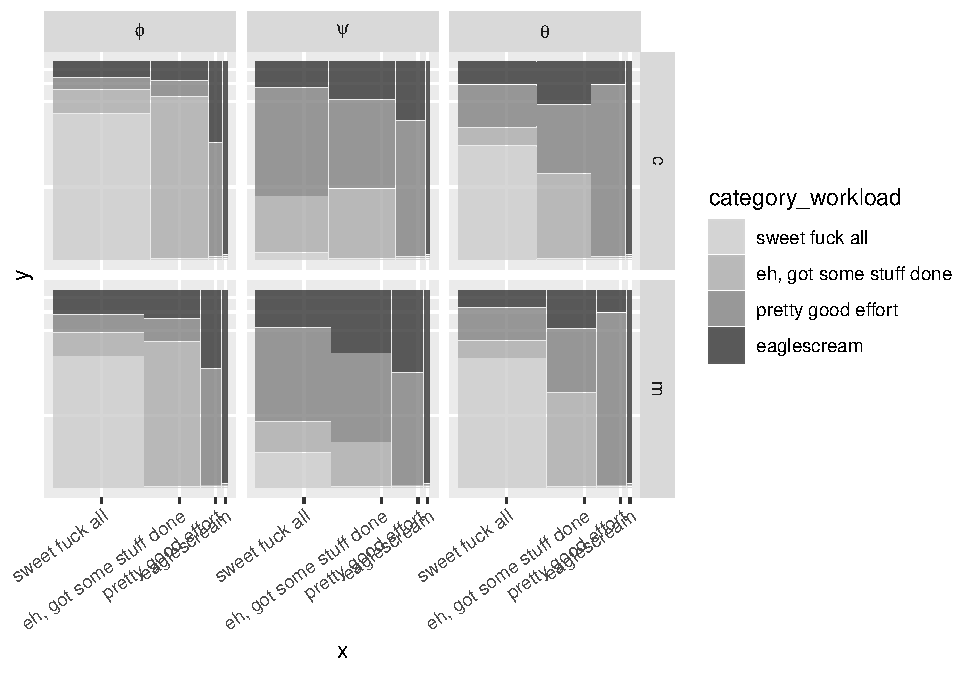
\includegraphics{lifeswork_files/figure-latex/vis-1.pdf}

\hypertarget{distribution-of-hrs-spent-per-day-per-category}{%
\section{distribution of hrs spent per day per category}\label{distribution-of-hrs-spent-per-day-per-category}}

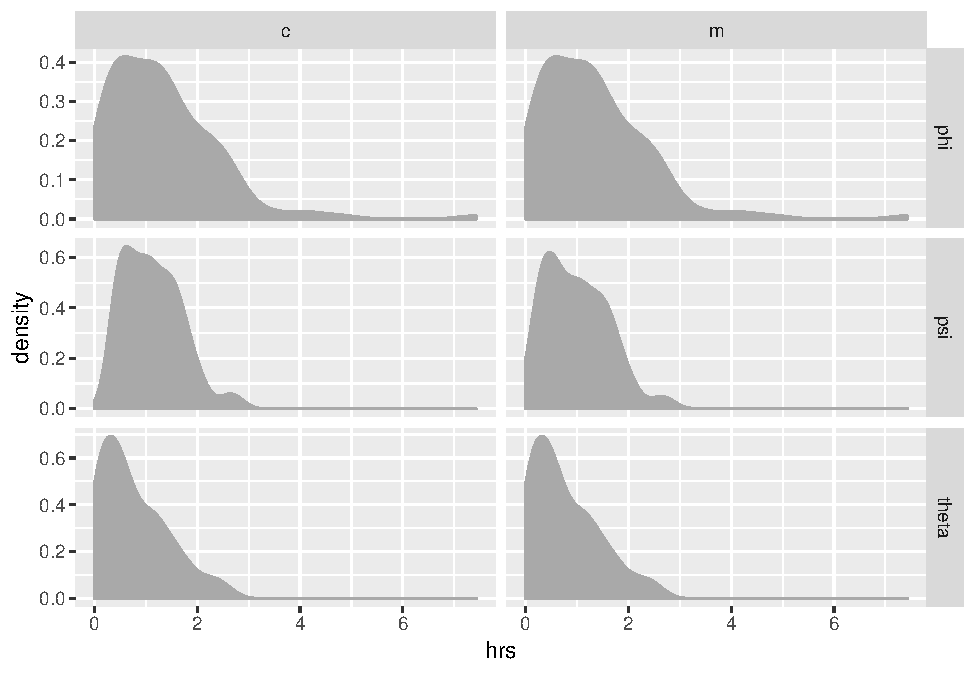
\includegraphics{lifeswork_files/figure-latex/density periods-1.pdf}

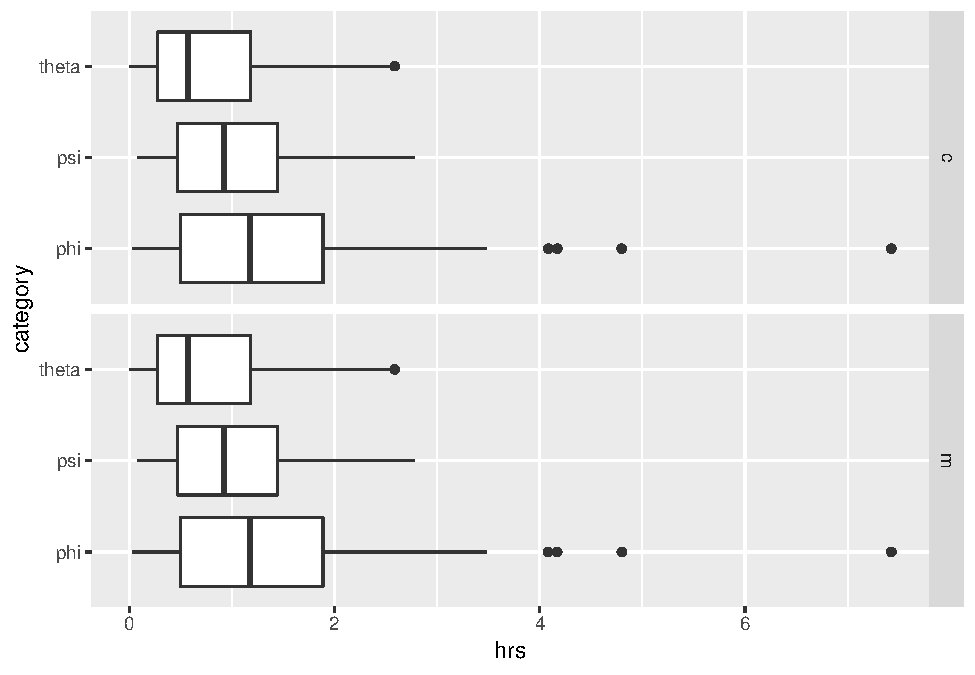
\includegraphics{lifeswork_files/figure-latex/boxplots categories-1.pdf}

\hypertarget{rituals}{%
\chapter{rituals}\label{rituals}}

\hypertarget{instantiate}{%
\section{instantiate}\label{instantiate}}

Start each \href{https://study.com/academy/lesson/german-days-of-the-week.html}{day} by drawing up a \protect\hyperlink{day-view}{day view}.

Begin the daily log, and add priority (\(*\)) \protect\hyperlink{daily-tasks}{daily tasks}.

\hypertarget{day-view}{%
\section{day view}\label{day-view}}

\begin{longtable}[]{@{}lll@{}}
\toprule
tracker & position & description\tabularnewline
\midrule
\endhead
goals & top left & pom goals\tabularnewline
poms & next to goals & track poms achieved\tabularnewline
projects & top right & one project/category\tabularnewline
\protect\hyperlink{order-of-events}{order of events} & below goals & live with intent\tabularnewline
task cycles & below projects & \(\varphi, \theta, \psi, \overline o\)\tabularnewline
\bottomrule
\end{longtable}

\hypertarget{daily-tasks}{%
\section{daily tasks}\label{daily-tasks}}

\hypertarget{section}{%
\subsection{\texorpdfstring{\(*\)}{*}}\label{section}}

\begin{tabular}{l|l|l|l|l|l}
\hline
priority & context & category & task & description & bump\\
\hline
\$*\$ & \$\textbackslash{}forall\$ & \$\textbackslash{}psi\$ & what is on fire? & What must be advanced today or very bad things will happen? What things will make me feel less anxious or possibly awesome if I advance them? & NA\\
\hline
\$*\$ & \$\textbackslash{}natural\$ & \$\textbackslash{}psi\$ & calendar & check day, week, month; note events of the day; upcoming deadlines & NA\\
\hline
\$*\$ & \$\textbackslash{}natural\$ & \$\textbackslash{}psi\$ & inboxes & email, 3c2 , handbag, unpack suitcase & NA\\
\hline
\$*\$ & \$\textbackslash{}sharp\$ & \$\textbackslash{}psi\$ & pill & take medication & NA\\
\hline
\end{tabular}

\hypertarget{sim}{%
\subsection{\texorpdfstring{\(\sim\)}{\textbackslash{}sim}}\label{sim}}

\begin{tabular}{l|l|l|l|l|l}
\hline
priority & context & category & task & description & bump\\
\hline
\$\textbackslash{}sim\$ & \$\textbackslash{}forall\$ & \$\textbackslash{}psi\$ & monthly log & check list for anything that is on fire & NA\\
\hline
\$\textbackslash{}sim\$ & \$\textbackslash{}forall\$ & \$\textbackslash{}psi\$ & thread & NA & NA\\
\hline
\$\textbackslash{}sim\$ & \$\textbackslash{}natural\$ & \$\textbackslash{}psi\$ & needs action & finish pom & NA\\
\hline
\$\textbackslash{}sim\$ & \$\textbackslash{}natural\$ & \$\textbackslash{}psi\$ & ynab & finish pom & NA\\
\hline
\end{tabular}

\hypertarget{varnothing}{%
\subsection{\texorpdfstring{\(\varnothing\)}{\textbackslash{}varnothing}}\label{varnothing}}

\begin{tabular}{l|l|l|l|l|l}
\hline
priority & context & category & task & description & bump\\
\hline
\$\textbackslash{}varnothing\$ & \$\textbackslash{}natural\$ & \$\textbackslash{}psi\$ & waiting & waiting emails & NA\\
\hline
\$\textbackslash{}varnothing\$ & \$\textbackslash{}natural\$ & \$\textbackslash{}theta\$ & export measures & download report into files, then email to myself, then download & NA\\
\hline
\end{tabular}

\hypertarget{pi}{%
\subsection{\texorpdfstring{\(\pi\)}{\textbackslash{}pi}}\label{pi}}

\begin{tabular}{l|l|l|l|l|l}
\hline
priority & context & category & task & description & bump\\
\hline
\$\textbackslash{}varnothing\$ & \$\textbackslash{}natural\$ & \$\textbackslash{}pi\$ & write to dani & check in with dani on slack & NA\\
\hline
\$\textbackslash{}varnothing\$ & \$\textbackslash{}sharp\$ & \$\textbackslash{}pi\$ & wash brushes & wash brushes & NA\\
\hline
\$\textbackslash{}varnothing\$ & \$\textbackslash{}sharp\$ & \$\textbackslash{}pi\$ & kitchen & clean kitchen & NA\\
\hline
\$\textbackslash{}varnothing\$ & \$\textbackslash{}sharp\$ & \$\textbackslash{}pi\$ & laundry & put away one basket of laundry & NA\\
\hline
\$\textbackslash{}varnothing\$ & \$\textbackslash{}sharp\$ & \$\textbackslash{}pi\$ & floors & vacuum & NA\\
\hline
\$\textbackslash{}varnothing\$ & \$\textbackslash{}sharp\$ & \$\textbackslash{}pi\$ & water plants & NA & NA\\
\hline
\end{tabular}

\hypertarget{review}{%
\section{\texorpdfstring{\textbf{review}}{review}}\label{review}}

\hypertarget{daily-log}{%
\subsection{daily log}\label{daily-log}}

This is the hard part.

Pare down to one active project per category and process daily log onto one page:

\begin{itemize}
\tightlist
\item
  if this project will take more than a day: migrate to \protect\hyperlink{monthly-log}{monthly log}, a collection tagged in the monthly log, or to GitHub issues
\item
  add \protect\hyperlink{signifiers}{signifiers}
\item
  log projects in \protect\hyperlink{day-view}{day view} tracker
\item
  add projects from \protect\hyperlink{monthly-log}{monthly log} if all \(*\) and \(\sim\) have been completed
\item
  aim to progress at least one \(*\) from the \protect\hyperlink{monthly-log}{monthly log}
\end{itemize}

\hypertarget{day-view-1}{%
\subsection{day view}\label{day-view-1}}

This is the sparkjoy bit.

\begin{itemize}
\tightlist
\item
  count poms
\item
  log goals
\item
  assign task cycles

  \begin{itemize}
  \tightlist
  \item
    exclude \(\varnothing\) categories with no \(*\) and \(\sim\) projects where current goal has already been met in poms by category
  \item
    always finish with scheduling review \(\overline o\)
  \item
    consider including a \href{https://en.wikipedia.org/wiki/Marie_Kondo}{sparkjoy} project
  \end{itemize}
\end{itemize}

\hypertarget{assess}{%
\subsection{assess}\label{assess}}

Calculate number of poms I can realistically do, the floor of
\[
14 - t - \frac 3 2 c
\]
where \(t\) denotes the number of hours of travel, and \(c\) the number of hours of \emph{community}, where the lattter includes teaching, outreach, and research collaborations. That, is I aim to draw a distinction between self-directed time, and time where I have the benefit of external motivations.

\begin{Shaded}
\begin{Highlighting}[]
\CommentTok{# output as of this update}
\NormalTok{dontpanic}\OperatorTok{::}\KeywordTok{calculate_pom_goal}\NormalTok{(}
  \DataTypeTok{travel_hrs =} \DecValTok{0}\NormalTok{, }\CommentTok{# no travel today}
  \DataTypeTok{community_hrs =} \DecValTok{0} \CommentTok{# no teaching, meetings today}
\NormalTok{)}
\end{Highlighting}
\end{Shaded}

\begin{verbatim}
## 
## aim to get 14 poms done today
\end{verbatim}

\begin{verbatim}
## # A tibble: 3 x 6
##   workload   phi theta   psi total aim_for
##   <chr>    <int> <int> <int> <int> <lgl>  
## 1 light        2     1     1     4 TRUE   
## 2 moderate     4     2     2     8 TRUE   
## 3 hardcore     6     4     4    14 TRUE
\end{verbatim}

\hypertarget{minibreak-peeps}{%
\subsection{minibreak peeps}\label{minibreak-peeps}}

\begin{itemize}
\tightlist
\item
  social media \& slack
\end{itemize}

\hypertarget{task-cycle}{%
\section{task cycle}\label{task-cycle}}

\begin{longtable}[]{@{}ll@{}}
\toprule
shorthand & description\tabularnewline
\midrule
\endhead
\(\forall *\) & complete all priority (\(*\)) tasks\tabularnewline
\(\sim \geqslant 1\) & complete at least one anxiety (\(\sim\)) task\tabularnewline
\(\varnothing \geqslant 0\) & complete any or none of the untagged tasks\tabularnewline
\(\cdot \geqslant 1\) & write down as many next actions as I can think of\tabularnewline
\(\overline o\) & \protect\hyperlink{review}{review}\tabularnewline
\bottomrule
\end{longtable}

\hypertarget{monthly-log}{%
\section{monthly log}\label{monthly-log}}

List of projects that will take longer than a day.

\hypertarget{pom-goals}{%
\section{pom goals}\label{pom-goals}}

pom := 20 minutes

\begin{tabular}{l|r|r|r|r}
\hline
workload & phi & theta & psi & exercise\\
\hline
light & 2 & 1 & 1 & 1\\
\hline
moderate & 4 & 2 & 2 & 2\\
\hline
hardcore & 6 & 4 & 4 & 3\\
\hline
\end{tabular}

\hypertarget{order-of-events}{%
\section{order of events}\label{order-of-events}}

Day begins with \protect\hyperlink{review}{review} \(\overline o\).

\hypertarget{workday}{%
\subsection{workday}\label{workday}}

Alternate events:

\begin{itemize}
\tightlist
\item
  \(\not n + 2\) poms
\item
  \(\pi\)
\end{itemize}

Around other events such as meetings.

\hypertarget{wake-up}{%
\subsection{wake up}\label{wake-up}}

\begin{itemize}
\tightlist
\item
  wake up
\item
  {[}read{]}
\item
  wash \& dress
\item
  {[}yoga{]}
\item
  \protect\hypertarget{day-view}{}{day view}
\item
  {[}yoga{]}
\end{itemize}

\hypertarget{evening}{%
\subsection{evening}\label{evening}}

\begin{itemize}
\tightlist
\item
  bathtime + reading
\item
  bed
\end{itemize}

\hypertarget{signifiers}{%
\section{signifiers}\label{signifiers}}

\begin{quote}
todo: create a signifiers sheet
\end{quote}

\begin{tabular}{l|l|r}
\hline
signifier & meaning & position\\
\hline
\$\textbackslash{}eigthnote\$ & today & 4\\
\hline
\$*\$ & priority & 5\\
\hline
\$i, ii, \textbackslash{}dots\$ & project & 4\\
\hline
\$\textbackslash{}sim\$ & anxiety & 5\\
\hline
\$\textbackslash{}cdot\$ & task & 1\\
\hline
\$\textbackslash{}varphi\$ & research & 2\\
\hline
\$\textbackslash{}theta\$ & skills & 2\\
\hline
\$\textbackslash{}psi\$ & busywork & 2\\
\hline
\$NA\$ & project & 3\\
\hline
\$NA\$ & look into & 3\\
\hline
\$\textbackslash{}natural\$ & on computer & 2\\
\hline
\$o\$ & event & 1\\
\hline
\$\textbackslash{}overline o\$ & review & 1\\
\hline
\$NA\$ & more than a day & 2\\
\hline
\end{tabular}

\hypertarget{playlists}{%
\section{playlists}\label{playlists}}

\hypertarget{for-the-good-days}{%
\subsection{for the good days}\label{for-the-good-days}}

\hypertarget{for-the-not-so-good-days}{%
\subsection{for the not so good days}\label{for-the-not-so-good-days}}

\hypertarget{ruminations}{%
\chapter{ruminations}\label{ruminations}}

\hypertarget{daily-projects}{%
\section{daily projects}\label{daily-projects}}

If a project is logged in the \protect\hypertarget{daily-log}{}{daily-log} then I am committing to finishing it today.

\hypertarget{pomodoros}{%
\section{pomodoros}\label{pomodoros}}

20 minutes seems to be the amount of time I can reasonably expect myself to focus unbroken.

\hypertarget{lowtech}{%
\section{lowtech}\label{lowtech}}

Keep what can be kept on paper, on paper. Keeps screens free of clutter and helps me focus.

\hypertarget{work-with-intent}{%
\section{work with intent}\label{work-with-intent}}

This term is adopted from a piano teacher that I studied under, that I subsequently adapted into my own teaching. She encouraged me to \emph{practice with intent}; that is, play what you intend to play. I found this to be particularly useful for discouraging my students, and myself, from the age-old pitfall of playing a piece of music until you make a mistake and stopping and playing that section over until you get it right. It's better to play \emph{through} the piece, which empowers you to adapt to mistakes you will inevitably play and, most importantly, not lose time. Oddly, it appeared to be a universal misconception, myself included, that without careful consideration, the attempt to \emph{get the notes right} inevitably means the \textbf{rhythm is wrong}, and thus you get nothing right after all. Best, therefore, to play through the piece. I use my bullet journal to help me focus on work with intent; I've found the simplicity of only timing work when I've written down what I intend to do has been extraordinarily powerful in helping me complete daunting tasks.

\hypertarget{mindfulness}{%
\section{documenting the system is mindful time}\label{mindfulness}}

I often update my system. I see this as productive mindfulness; it is both meditative, I enjoy making something I find aesthetically pleasing, and functional, the systems do help me work happier.

Something that really resonated with me about Cal Newport's \emph{Deep Work} was that my situation will change, and so, too, may what best facillitates flow. I will pick and choose elements from pomodoro, gtd, task switching, and so forth to achieve flow. Allowing this to be so flexible makes keeping track of my own system tricky at times.

todo: fix inconsistencies in audience across manuscript - should be to self

I am slowly automating the process of updates, where the manual process is ideally kept to tweaking a set of easy to navigate \href{https://docs.google.com/spreadsheets/d/1hv7pkBGu8XQQOIBbBt1_1LvKGBR7zTdQYCzogrv3hz0/edit?usp=sharing}{googlesheets} which are scraped using the fabulous \texttt{googlesheets::} and rendered with \texttt{bookdown::}. It's exciting that using git, I can examine past systems.

todo: refs

This has a dual objective of providing a place to drop my thoughts, but also to test run \texttt{bookdown::}, as I will likely write my thesis in something this or \texttt{distill::}. Also, I think it'll level up my git-surfing skills.

I enjoy taking breaks from doing mathematics to document my system and analyse my productivity.

I often feel like it's about finding activities that are posisitive experiences \emph{and} productive in some way (for me, \(\varphi\), \(\theta\), \(\psi\), andn \(\pi\)). So, working on my system is \(\pi\).

\hypertarget{sim-beethoven-piano-sonata}{%
\section{\texorpdfstring{\(\sim\) beethoven piano sonata}{\textbackslash{}sim beethoven piano sonata}}\label{sim-beethoven-piano-sonata}}

todo:
\url{https://twitter.com/cantabile/status/1112145903203180544}

\bibliography{book.bib,packages.bib}


\end{document}
